\documentclass{article}

%%% PAGE DIMENSIONS
\usepackage{geometry}
\geometry{a4paper}
\geometry{margin=2cm}

%%% PACKAGES
\usepackage[authoryear]{natbib}
\bibliographystyle{besjournals}

\usepackage{makecell,booktabs}

\usepackage{setspace}
\doublespacing

\usepackage{graphicx}

\usepackage{tabularx}

\usepackage{multirow}

\usepackage[running]{lineno}

\usepackage{caption}
\captionsetup{justification=raggedright, singlelinecheck=false}
\usepackage[font=small,labelfont=bf,labelsep=space]{caption}

\usepackage{subcaption}
\captionsetup{justification=raggedright, singlelinecheck=false}
\usepackage[font=small,labelfont=bf,labelsep=space]{subcaption}

\usepackage{pgfplots}
\pgfplotsset{width=16cm}

\usepackage{amsmath}

\usepackage{pdflscape} %for landscape table

\usepackage{afterpage} %for Table on next page

%%% HEADERS and FOOTERS
\usepackage{fancyhdr}
\pagestyle{fancy}
\renewcommand{\headrulewidth}{0pt}
\lhead{}\chead{}\rhead{}
\lfoot{}\cfoot{\thepage}\rfoot{}

%%% SECTION TITLE APPEARANCE
\usepackage{sectsty}
\setcounter{secnumdepth}{-1}
\subsectionfont{\normalfont\fontsize{10}{15}\selectfont}
\DeclareMathSizes{10}{11}{9}{7}

%%% DEFINE NEW COMMANDS
\newcommand{\B}{\textbf}
\newcommand{\TL}{\textless}
\newcommand{\PRZ}{\text{Pr}\bigl( >\mid Z \mid \bigr)}
\newcommand{\head}[1]{\textnormal{\textbf{#1}}}

\newenvironment{nscenter}
 {\parskip=.75pt\par\nopagebreak\centering}
 {\par\noindent\ignorespacesafterend}

\makeatletter
\renewcommand{\fnum@figure}{Fig. \thefigure.}
\renewcommand{\fnum@table}{Table \thetable.}
\makeatother

\newcommand{\fillcaption}[1]{ %new command with the argument being the text of the caption
\textbf{Fig. \arabic{figure}:} #1 %Makes main figure number, concatenates it to legend
\addtocounter {figure} {1} %increments main figure count
}

%% FOR SUPPLEMENT SETTINGS
\newcommand{\beginsupplement}{%
        \setcounter{table}{0}
        \renewcommand{\thetable}{S\arabic{table}}%
        \setcounter{figure}{0}
        \renewcommand{\thefigure}{S\arabic{figure}}%
     }

\begin{document}


%%% DOCUMENT CONTENT
\title{Traits paper}
\author{Saras M. Windecker, Stacey M. Trevathan-Tackett, Nick Golding, Peter A. Vesk}
\date{April, 2018}
%\address[add1]{School of BioSciences, University of Melbourne, Parkville VIC 3056, Australia}
%\address[add2]{Centre for Integrative Ecology, Deakin University, 221 Burwood Hwy, Burwood VIC 3125, Australia}

\pgfplotsset{compat=1.9}

\section{Abstract}
fundamental study of biomass traits. these are measured in XX way. essentially orthogonal. they have a good theoretical link to decay. species vary by them. they are therefore potentially very useful - and can tell us something different about trait effects on ecosystem functions. 

this paper is not about establishing a mechanistic link. 


1. what is the issue?
Understanding the trends in litter decomposition is an important link to how plant communities impact carbon sequestration and other biogeochemical processes in soil. 

2. what has been done?
Comparative approaches use attributes of plant species, termed functional traits, in order to generalise plant community litter dynamics. In particular, dry matter content has been used to predict decay as it is a direct measure of the contribution of structural material. However traits such as dry matter content group dry weight material together, assuming that rather heterogenous material can be characterised by the same overall measure. 

3. this paper fills x gap


4. this is how we fill it
5. we found X
6. implications of X. 

\section{Introduction}

Functional traits are useful for identifying plant community response to environmental change and effect on ecosystem functions \citep{diaz2007,lavorel2002},laliberte. Functional traits have many predicted connections to soil carbon and other biogeochemical processes, particularly relevant to the global carbon cycle and sequestration of atmospheric CO2. Aboveground material contributes to soil carbon primarily via deposition of litter material \citep{valery2004}, and subsequent decomposition rates and processes of that material. Changes in community composition can affect soil carbon storage through changing the chemical and physical structure of litter \citep{liao2007}. Plant litter may become recalcitrant, or resistant to decay, in soil due to abiotic conditions such as oxygen availability, water levels, pH, and ambient nutrients, or biotic conditions, particularly the microbial and macroinvertebrate decomposer communities. However, litter characteristics, measured by traits, are strongly tied to decay rates in soil \citep{cornwell2008}. This study aims to examine traits linked to litter chemistry and structure. 

Decomposition research has found a variety of green leaf economic traits impact decomposition rate of both leaf \citetext{specific leaf area/leaf mass area and leaf nitrogen \citealp{devries2012,cornwell2008}, and leaf carbon \citealp{britson2016}} and litter material \citetext{litter carbon and dry matter content \citealp{freschet2012}}. These traits are part of the leaf economic spectrum (LES), which conceptualises a trade-off between nutrient acquisitive and nutrient conservative plant ecological strategies, based on a finding that nearly 3/4 of global variation in key leaf traits are captured by a single axis in multidimensional trait space \citep{wright2004}. This single axis of variation suggests species tend to be either highly productive, producing a large volume of high-quality litter that provide a quick return on C, N, and P investment, or highly persistent, producing fewer low-quality leaves that have a slower return on investment **different citation here. Productive, nutrient acquisitive species tend to have high sla, low ldmc, high n, and low c, and decompose fast, accumulating easily decomposed, labile tissue high in solubles. Persistent, nutrient conservative species tend to have low sla, high ldmc, low, and high c, and decompose slow, accumulating denser tissue. Specific leaf area and dry matter content are not direct measures of litter chemistry however, as they are calculated using leaf/litter dry weight, which itself encompasses a range of tissue material including nutrients, proteins, carbon, and others (Fig 1). Abiotic and biotic conditions mean even labile tissue can become recalcitrant in a particular environment, but tissue high in chemically complex carbon forms, such as lignin, are much more likely to become recalcitrant in soil. So, while these economic spectrum traits have provided strong correlation to decay rate, they are not direct measures of tissue carbon chemistry. 

We have long known that lignin in particular is a strong predictor for decay rate \citealp{britson2016,cornwell2008,makkonen2012,freschet2012a,freschet2012}; composed of three kinds of heavily-linked benzene-propane, thermal stability of lignin is high, and as such it is more difficult to decompose. While organic biomass consists of a range of material, lignin joins hemicellulose and cellulose as three primary components collectively termed `lignocellulosic biomass’ distinct structure that decompose at different rates in different conditions. Hemicellulose is composed of simple sugar monomers with random, amorphous structure. These have little strength and are easily hydrolysed \citep{muller-hagedorn2007}. Cellulose forms long polymers of glucose units without many branches, making these linear crystals more stable than simple sugars. Some decomposition work has examined the ability of other biomass components to predict decay \citetext{including cellulose \citealp{britson2016}, and a range of other organic compounds identified by infrared spectroscopy \citealp{lang2009}}, but there has not been a clear/consistent examination of biomass components in species and across trait space. The approximate decomposition of litter tissue suggests the lignocellulosic composition of leaf carbon may not be related to SLA or to the LES at all.

Economic spectrum traits generally accepted methodologies for their measurement, complying with guiding principles of trait measurement, which suggest methods should be straightforward and reproducible \citep{perez-harguindeguy2013}. Wet chemistry assays are the most common methods to measure biomass components in tissue, but are costly in environmental impact, time, and funds. A potential alternative is `thermogravimetric analysis’ (TGA), during which mass is recorded while subjected to rising temperatures; mass loss over this thermal gradient can be regarded as the sum of the degradation of the main components of that biomass \citep{hu2016,barneto2009,yang2006,cheng2015,perejon2011,orfao2001chen2017,muller-hagedorn2007}. Mass fractions of each of three primary components - hemicelluloses, cellulose, and lignin - can be mathematically deconvoluted from the multi-peaked decay rate curve, a method which has been validated by studies comparing estimates to experimental measurements \citep{yang2006,barneto2009}. Much of the published literature use software to conduct the deconvolution \citetext{for example OriginPro \citealp{chen2017}, PeakFit \citealp{strandberg2017,perejon2011}, Fityk \citealp{perejon2011}, or Datafit \citealp{cheng2015}}, so while it has been used to identify species' recalcitrance \citetext{for example in seagrasses \citealp{trevathan-tackett2015}, and eucaplyts \citealp{orfao2001}}, the deconvolution procedure can be challenging to replicate and has not been deeply examined for its application to comparative studies. 

In the present study, we examine and demonstrate the application of TGA for estimating the partitioning of litter carbon, into what we call ‘biomass traits’, in 29 wetland species, using an open source mixture model we developed for the deconvolution. In the present study, we examine and demonstrate the application of TGA for estimating the partitioning of litter carbon, into what we call ‘biomass traits’, in 29 wetland species, using an open source mixture model we developed for the deconvolution. We measure a range of functional traits included in the LES and related to litter decomposition in addition to our measured biomass traits, to: 
1.	assess the relationship and coordination of carbon components to the existing trait economic spectrum
2.	and guide whether we can use that spectrum to generalise carbon investment in biomass tissue.


\begin{figure}[ht]
	\centering
	\scalebox{0.9}
	{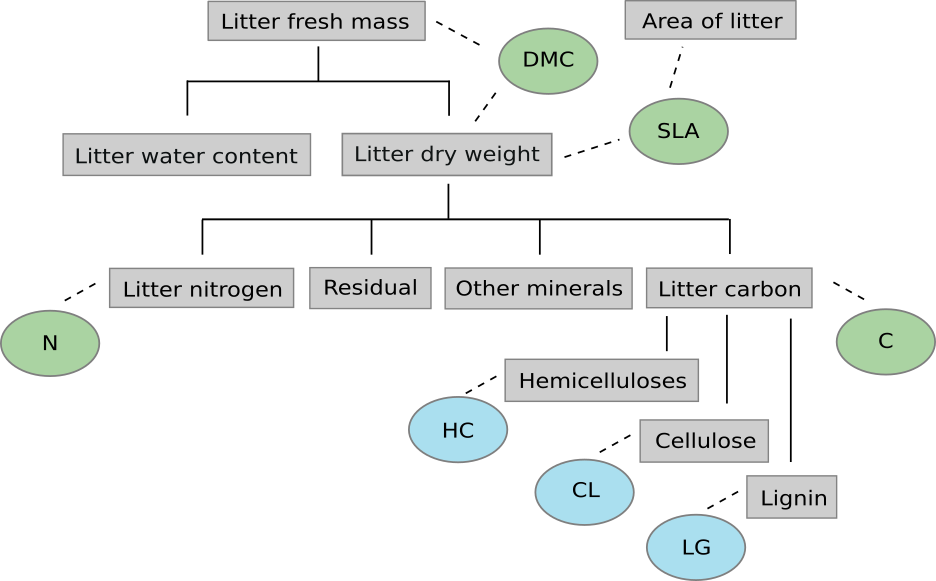
\includegraphics[width=\textwidth]{figs/trait_flowchart.png}}
	\caption{Breakdown of the relationships between functional traits related to litter recalcitrance examined in this study. Rectangles represent attributes or components of litter, ellipses represent traits: dry matter content (DMC), specific litter area (SLA), litter nitrogen (N), litter carbon (C), litter hemicelluloses (HC), litter cellulose (CL), and litter lignin (LG).}
	\label{Fig:flowchart}
\end{figure}

\section{Materials and Methods}

\subsection{Litter collection}
In late austral summer 2016, we collected litter of 29 wetland plant species from ten sites in the southern portion of the Australian state of Victoria. To avoid the effects of seasonal variation, all leaves were collected at the end of the growing season, while fully mature. Species covered a range of functional communities: graminoids (n = 15), forbs (n = 9), woody species (trees, n = 5; shrub n = 1), and one non-vascular bryophyte. A target species list was organised before fieldwork to include functional types of interest, based upon existence of known species at three diverse wetlands that had been previously surveyed. We planned to collect a representative range of species at only three sites to reduce the variability introduced from local site conditions. This species list was modified slightly during litter collection due to availability of target species. When a target species was identified, we collected ten robust, well-grown individuals of each species at least 5 m apart along a linear transect within a single site, per recommendations in the revised handbook for functional traits \citep{perez-harguindeguy2013}. Litter was stored in moist plastic bags in dark coolers during transportation and maintained in a dark refrigerated room, no more than 24 hours, until they could be weighed. 

Since the aim of this study was to examine traits related to litter effects on decomposition and soil carbon storage, we included in trait measurement any biomass that would contribute to litter. For graminoids (grasses, rushes, and sedges; growth form 'G' hereafter), litter included the photosynthetic culm, leaves, and involucral leaves (where existent), but not the inflorescence or roots. For herbs and ferns (grouped as forbs, termed 'F' hereafter), litter included the entire body of the plant excluding the flower if present, and the roots. For tree species (growth form 'T'), leaves and petioles, leaflets and rachis (in \textit{Acacia dealbata}), but not seeds, flowers, or stems were included. For the bryophyte (growth form 'NV'), the entire individual was included, and for the shrub \textit{Meuhlenbeckia florulenta} (growth form 'S'), leaves as well as green portions of the stem were included. Empirical work has found reasonable coordination of traits associated of traits among different plant parts \citep[for example, leaves and stem,][]{reich2014,jackson2013}, and similar patterns with respect to effect on decay rate for traits measured on leaf and litter tissue \citep{cornwell2008}, so for the purposes of examining litter quality, this is a reasonable choice. 

\begin{table}[ht]
	\caption{Selected traits and measurement methods.}
	\label{Tab:traits}
	\centering
	\small
	\begin{tabularx}{\textwidth}{lllX}
        		\toprule
        		Abbreviation & Trait & Units & Method \\
        		\midrule
		SLA & Specific litter area & m$^2$/g & One-sided area of fresh litter (m$^2$) divided by its oven-dry mass (g) \\
		DMC & Litter dry matter content & mg/g & Oven-dry litter mass (mg) divided by water-saturated fresh litter mass (g) \\
		N & Litter nitrogen content & wt\% & Weight \% elemental N in dry litter mass measured with LECO Elemental Analyser \\
		C & Litter carbon content & wt\% & Weight \% elemental C in dry litter mass measured with LECO Elemental Analyser \\
		HC & Litter hemicelluloses & wt\% & Weight \% hemicelluloses in dry litter mass from thermogravimetric analysis \\
		CL & Litter cellulose & wt\% & Weight \% cellulose in dry litter mass from thermogravimetric analysis \\
		LG & Litter lignin & wt\% & Weight \% lignin in dry litter mass from thermogravimetric analysis \\
        		\bottomrule
	\end{tabularx}
\end{table}

\subsection{Economic spectrum traits}
Specific litter area (SLA) and litter dry matter content (DMC) were measured per recommendations in the functional trait handbook \citep{perez-harguindeguy2013} with the exception of the plant parts included, as discussed previously. Trait values were expressed as the mean of the ten replicates for each species. Litter from all ten samples were then pooled and ground in a XXX to XXX size, and approximately 150 mg of dried ground litter was analysed for litter nitrogen (N) and litter carbon content (C) in a LECO Elemental Analyser, using an ethanol standard (Table~\ref{Tab:traits}). 

\subsection{Lignocellulosic biomass method}
We estimated mass fractions of lignocellulosic biomass components from the outputs of thermogravimetric analysis (TGA). During TGA, biomass samples are heated in a linear temperature program, the primary result of which is a graph of remaining weight v. temperature (Fig.~\ref{Fig:TG}). In this study, Dry litter samples used to measure economic spectrum traits were pooled and ground, 10\textendash20 mg samples of which were passed through the TGA-FTIR where they were pyrolysed in an N$_2$ environment from 30 to 800 $^{\circ}$C at a temperature ramp of 10 $^{\circ}$C/min (Table~\ref{Tab:traits}). 

The negative first derivative of the thermogravimetric (DTG) curve depicts rate of mass loss over temperature increase (Fig.~\ref{Fig:DTG}). This multi-peaked plot has three main phases \citep{orfao2001}: 

\begin{enumerate}
	\item A small but pronounced peak of moisture and light volatile evolution until approximately \textless120 $^{\circ}$C.
	\item A wide range of high mass loss, caused by devolatilisation of lignocellulosic biomass components (hemicelluloses, cellulose, and lignin) between approximately 120\textendash650 $^{\circ}$C.
	\item A final period of little mass loss due to decomposition of carbonaceous material associated with the inorganic fraction retained in char residue after approximately \textgreater650 $^{\circ}$C.
\end{enumerate}

\begin{figure}
\centering
	\begin{subfigure}[!ht]{0.3\textwidth}
		
\includegraphics[width=\textwidth]{figs/TG.png}
		\phantomcaption{\label{Fig:TG}}
	\end{subfigure}\hfill
	\begin{subfigure}[!ht]{0.3\textwidth}
		
\includegraphics[width=\textwidth]{figs/DTG.png}
		\phantomcaption{\label{Fig:DTG}}
	\end{subfigure}\hfill
	\begin{subfigure}[!ht]{0.3\textwidth}
		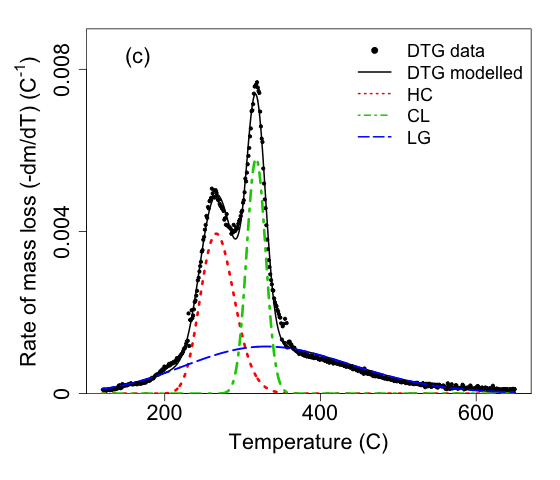
\includegraphics[width=\textwidth]{figs/DTG-mixture.png}
		\phantomcaption{\label{Fig:DTGmixture}}
	\end{subfigure}
	\caption{Detailed exploration of thermogravimetric analysis and mixture modelling using \textit{Juncus amabilis} as an example species: Mass loss curve, where heating rate = 10$^\circ$C/min (a); Negative first derivative thermogravimetric curve displaying mass loss rate across entire temperature range (b); Output of deconvolution of negative derivative thermogravimetric curve (c). Rate of mass loss (DTG) values scaled by initial mass of sample.}
	\label{Fig:TGAmethod}
\end{figure}

Since the overall DTG curve also represents the loss of extractives, water, inorganic matter, and volatiles, to assist us in isolating the biomass components, we crop the DTG data between 120 $^{\circ}$C (below which is mostly dehydration) and 650 $^{\circ}$C (above which is mostly extractives and volatiles) \citep{hu2016,samtani2002}. The DTG curve, cropped to the second phase, can be used to estimate mass fractions of the three main components of biomass (hemicelluloses, cellulose, and lignin), by `deconvoluting', or separating, the multi-peaked curve into its constituent parts (Fig~\ref{Fig:DTGmixture}). 

While the biomass decomposition curves for the three primary components overlap in the DTG curve, research has found little interaction between the biomass fractions during thermal volatilisation, indicating that decomposition of one component does not interfere with decomposition of the others: they decompose reasonably independently \citep{yang2006}. Because we can assume the three main components decompose independently, the mass ($m$) loss equation can be expressed as the sum of $n$ independent reactions, as follows \citep{orfao2001}:

\begin{gather}\label{eqn:mixture_model}
	-\frac{dm}{dT} = \sum\limits_{i=1}^n c_i\frac{d\alpha_{i}}{dT}\\
	m = \frac{M_T}{M_0}\\
	c_i = M_{0i} - M_{\infty i}
\end{gather}

where mass ($m$) is expressed as a fraction of mass at temperature $T$ ($M_T$) in initial sample mass ($M_0$), $c_i$ is the mass of component $i$ that is decayed of $n$ independent reactions, $M_{0i}$ and $M_{\infty i}$ are the mass of the initial and final pyrolysis of the $i$-th component, respectively. While most of my curves could be described with only $n$ = 3 peaks, corresponding to a single hemicelluose, cellulose, and lignin peak, for some species a second hemicellulose peak was observed at a lower temperature, resulting in $n$ = 4 independent peaks \citep[see also][]{chen2017,muller-hagedorn2007}, since the soluble carbohydrates in plant tissue can take many forms, including xylan, amylose, etc, which may degrade primarily in different temperature regions. 

In order to use DTG data to estimate the mass fractions of carbon forms we must resolve the form of the independent reactions ($\frac{d\alpha_{i}}{dT}$). Many different functions have been proposed, including the asymmetric bi-Gaussian \citep{sun2015}, logistic \citep{barbadillo2007}, Weibull \citep{cai2007}, asymmetric double sigmoidal \citep{chen2017}, and the Fraser-Suzuki function \citep{perejon2011,hu2016}. Comparisons of several techniques \citep{svoboda2013,perejon2011,cheng2015} found that the Fraser-Suzuki function best fit these kinetic curves, since it allows for asymmetry, and has been used to successfully produce consistent and accurate biomass estimates. A parametric examination of the Fraser-Suzuki function can be found in Fig.~\ref{Fig:fs_simulation}. 

We can therefore use the Fraser-Suzuki function to describe the rate expression, $\frac{d\alpha_{i}}{dT}$, which is the derivative of $\alpha_i$, the conversion of mass at a given temperature ($M_{Ti}$), from the initial ($M_{0i}$), given total mass lost between the initial and final ($M_{\infty i}$) temperature for each curve. The rate expression for a single curve can thus be written as follows:

\begin{gather}\label{eqn:fs_function}
	\frac{d\alpha_i}{dT} = h_i\ exp\bigg\{-\frac{ln2}{s_i^2}\Big[ln\Big(1 + 2s_i \frac{T - p_i}{w_i}\Big)\Big]^2\bigg\}\\
	\alpha_i = \frac{M_{0i} - M_{Ti}}{M_{0i} - M_{\infty i}}
\end{gather}

where T is temperature ($^\circ$C), and the parameters h$_i$, s$_i$, p$_i$, and w$_i$ are height, skew, position, and width of the curve, respectively. In total the model estimates 12 or 16 parameters, one for each parameter for either three or four primary components. Starting values were selected based on curves depicted in the literature. Hemicelluloses are made of simple sugars, and are easily hydrolysed; these carbon components decay in reasonably narrow bands at lower temperature intervals \citep{barneto2009,muller-hagedorn2007}, so we set starting values to 210 and 270 for position and 50 each for width. Linear cellulose crystals are more resistant to decay than hemicelluloses, decaying at a higher temperature (starting position set to 310), but decaying more rapidly once peak temperatures are reached (starting width set to 30). Since lignin typically decays over a wide temperature interval, and in general dominates mass loss above 400 $^{\circ}$C \citep{chen2015,cai2013,cai2014,varhegyi2011}, starting values for its position and width were 410 and 200, respectively. 

Starting values are first passed through an optimiser to select starting values based on minimising the root mean squared error (Eq.~\ref{eqn:obj_function}), for use in non-linear least-squares fit using modelling package, \textit{minpack.lm} \citep{minpack.lm}. \citet{cheng2015} similarly used non-linear optimisation using minimum residual sum of squares to fit the rate expression. 

\begin{gather}\label{eqn:obj_function}
	RMSE = \sqrt{\frac{1}{n} \sum_{j=1}^{n} (y_j - \hat{y}_j)^2}
\end{gather}

The weight of each component in the overall sample can then be calculated by integrating under each component's curve. These values are expressed as weight \%. 

\begin{gather}\label{eqn:integration}
	m_i = \int_{120}^{650} h_i\ exp\bigg\{-\frac{ln2}{s_i^2}\Big[ln\Big(1 + 2s_i \frac{T - p_i}{w_i}\Big)\Big]^2\bigg\} dT
\end{gather}

We infer that the curve located around 250\textendash270 $^\circ$C corresponds to primary hemicelluloses (HC-2), 310\textendash330 $^\circ$C to cellulose (CL), and 330\textendash350 $^\circ$C to lignin (LG). If present, the fourth curve located below 200 $^\circ$C corresponds to the most simple hemicelluloses (HC-1). In later analyses the hemicelluloses trait (HC) refers to the sum of HC-2 and HC-1, if present. The mixture model and associated analyses (Eq.~\ref{eqn:mixture_model}) were fit using functions made available in the R package \textit{deconvolve} \citep{deconvolve}. 

\subsection{Analysis}
In order to examine relationships between traits and groupings, simple boxplots were utilised. To compare the biomass traits with the LES traits, a Principal Components Analysis (PCA) and simple pair-wise comparisons were used. PCA used the eigenvalues of the correlation matrix of traits. 

In order to test the structure of our mixture model, we ran the single curve deconvolution on pure cellulose and pure lignin samples using the same protocol as for our biomass samples. In order to estimate the uncertainty of the weight predictions for the biomass samples, we calculated the 95\% interval for the weight estimates across a random sample of parameter estimates, drawn in proportion to their likelihood. We assumed a truncated multivariate normal distribution, since height, position, and width parameters are constrained to positive values, using the package \textit{tmvtnorm} \citep{tmvtnorm}. 

To examine evolutionary patterns in trait values among these species, we created a phylogeny, and compared patristic distance (sum of branch lengths) to trait distance using the Mantel Test. Genetic sequences for the rbcL and matK gene were accessed from GenBank (Table~\ref{Tab:genbank}). In some cases both gene regions were not available for all species, so a sequence of a species from the same genus was used. Sequences for each gene were aligned in Geneious 10.2.3 \citep{kearse2012} using the MAFFT \citep{katoh2013} plugin, the alignments were trimmed to reduce missing data, and subsequently concatenated. The phylogeny was constructed with the MrBayes \citep{ronquist2012} plugin in Geneious using the following parameters: GTR+I+G model, the genes partitions were unlinked, and the chain was run for 1 million generations with a 100,000 generation burn-in. A 50\% majority rule consensus tree was obtained and used for subsequent analyses. 

Patristic distances were calculated using the \textit{adephylo} package \citep{adephylo}. We executed the Mantel Test using the \textit{ade4} package \citep{ade4}, in which the two distance matrices are subjected to 99 random permutations, and assessed significance at $P$ \textless 0.05. 

All analyses were conducted within the statistical computing environment, R \citep{R}, and R code for this paper are available at \citep{biomass_traits}.

\section{Results}
\subsection{Partitioning of litter carbon}
Across all species, the results of the negative first derivative thermogravimetric (DTG) deconvolution provided three or four consistent peaks (Fig.~\ref{Fig:tga_all}). \textbf{CHECK Three species had an additional hemicellulose peak below 220 $^{\circ}$C (\textit{Cycnogeton procerum}, \textit{Cyperus eragrostis}, and \textit{Marsilea drumondii}.} The lower hemicellulose peak occurred at a mean temperature of 184.7 $^\circ$C, the higher peak, common among all species, occurred at a mean temperature of 264.4 $^{\circ}$C with a standard deviation of 12.5 $^{\circ}$C (Table~\ref{Tab:parameters}). Our cellulose curves across species peaked at a mean of 318.2 $^{\circ}$C (SD 8.8 $^{\circ}$C) and had the narrowest width (34.1 $^{\circ}$C), compared to the two hemicelluloses (55.9 and 63.1 $^{\circ}$C, respectively), or to lignin (243.2 $^{\circ}$C; Table~\ref{Tab:parameters}). Lignin curves, in addition to being the widest, also occurred at the highest temperature (mean 334.8 $^{\circ}$C, SD 11.8 $^{\circ}$C; Table~\ref{Tab:parameters}). 

Add in standards work here. what even are the values? 


While width and positions of component curves were consistent, height variance between species and among growth forms dominated estimated differences in wt\% of biomass components. Graminoid species, with the notable exception of the fleshy aquatic \textit{Cycnogeton procerum} generally displayed higher cellulose peaks (mean 0.0058 $^\circ$C$^{-1}$) than forbs (0.0029 $^\circ$C$^{-1}$), or trees (0.0022 $^\circ$C$^{-1}$; Fig.~\ref{Fig:tga_all}, Table~\ref{Tab:parameters}). This is mirrored in the higher overall wt\% cellulose for graminoids (Fig.~\ref{Fig:boxplots}). Similarly, there is a very clear increase in mean height of the lignin curve for the four tree species (mean 0.0021, compared to 0.0011 (G), and 0.0012 $^\circ$C$^{-1}$ (F); Fig.~\ref{Fig:tga_all}, Table~\ref{Tab:parameters}) that has a clear tie to higher wt\% of lignin (49.8 (T) compared to 29.4 (G), and 31.6 wt\% (F); Fig.~\ref{Fig:boxplots}). 

Overall, the lowest wt\% of lignin was found in the diminutive aquatic grass, \textit{Paspalum distichum} (22.2 wt\%; Table~\ref{Tab:speciestraits}), and highest for the woody acacia, \textit{Acacia dealbata} (55.7 wt\%; Table~\ref{Tab:speciestraits}). Hemicelluloses followed a reverse pattern, in which \textit{A. dealbata} had the lowest total wt\% and the invasive sedge \textit{Cyperus eragrostis} had the highest (7.8 and 31.1 wt\%; Table~\ref{Tab:speciestraits}). Cellulose was lowest in the Australian river red gum, \textit{Eucalyptus camaldulensis} (7.2 wt\%; Table~\ref{Tab:speciestraits}), and highest again for \textit{P. distichum} (26.5 wt\%; Table~\ref{Tab:speciestraits}). 

\begin{figure}[!ht]
	\centering
	{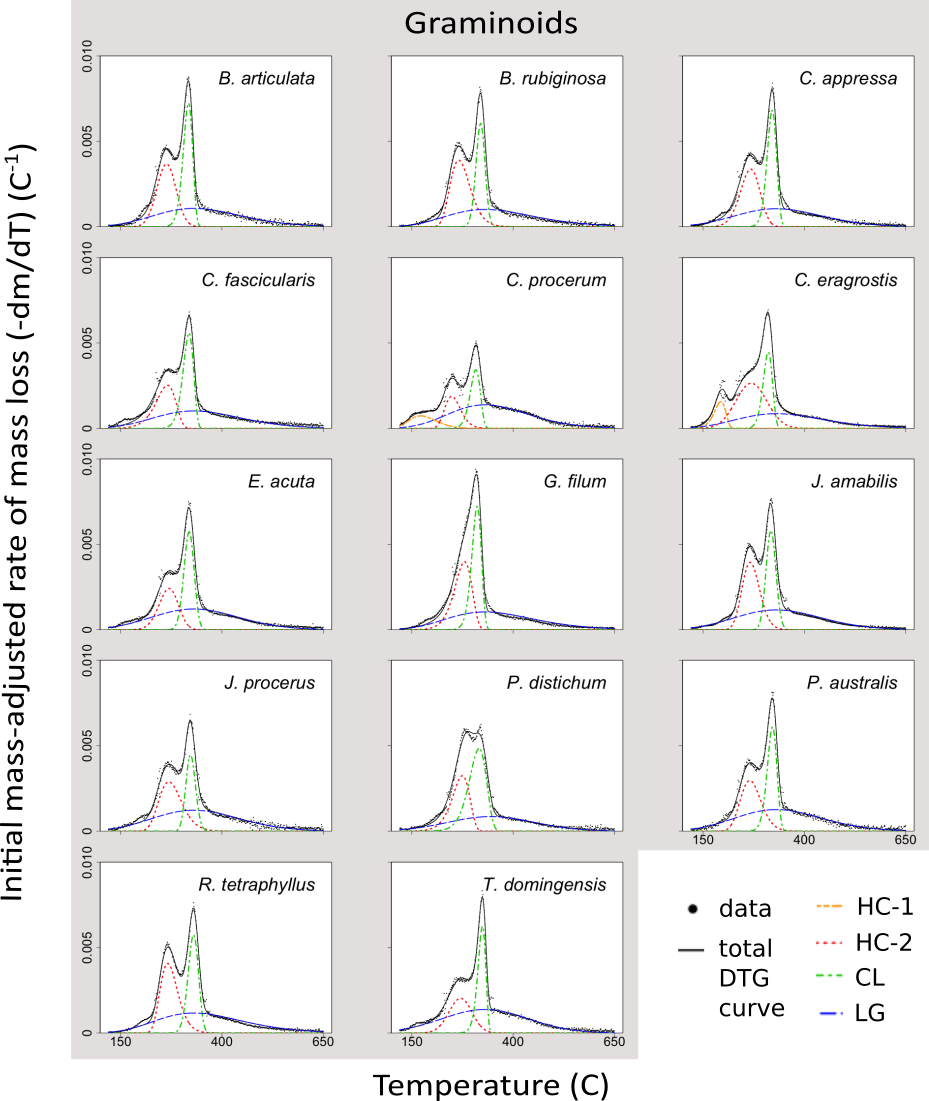
\includegraphics[width=\textwidth]{figs/TGA_fig_gram.png}}
	\caption{Output of deconvolution of thermogravimetric analysis curves. Rate of mass loss (DTG) values scaled by initial mass of sample.}
	\label{Fig:tga_all}
\end{figure}

\begin{figure}
	\ContinuedFloat
	\centering
	{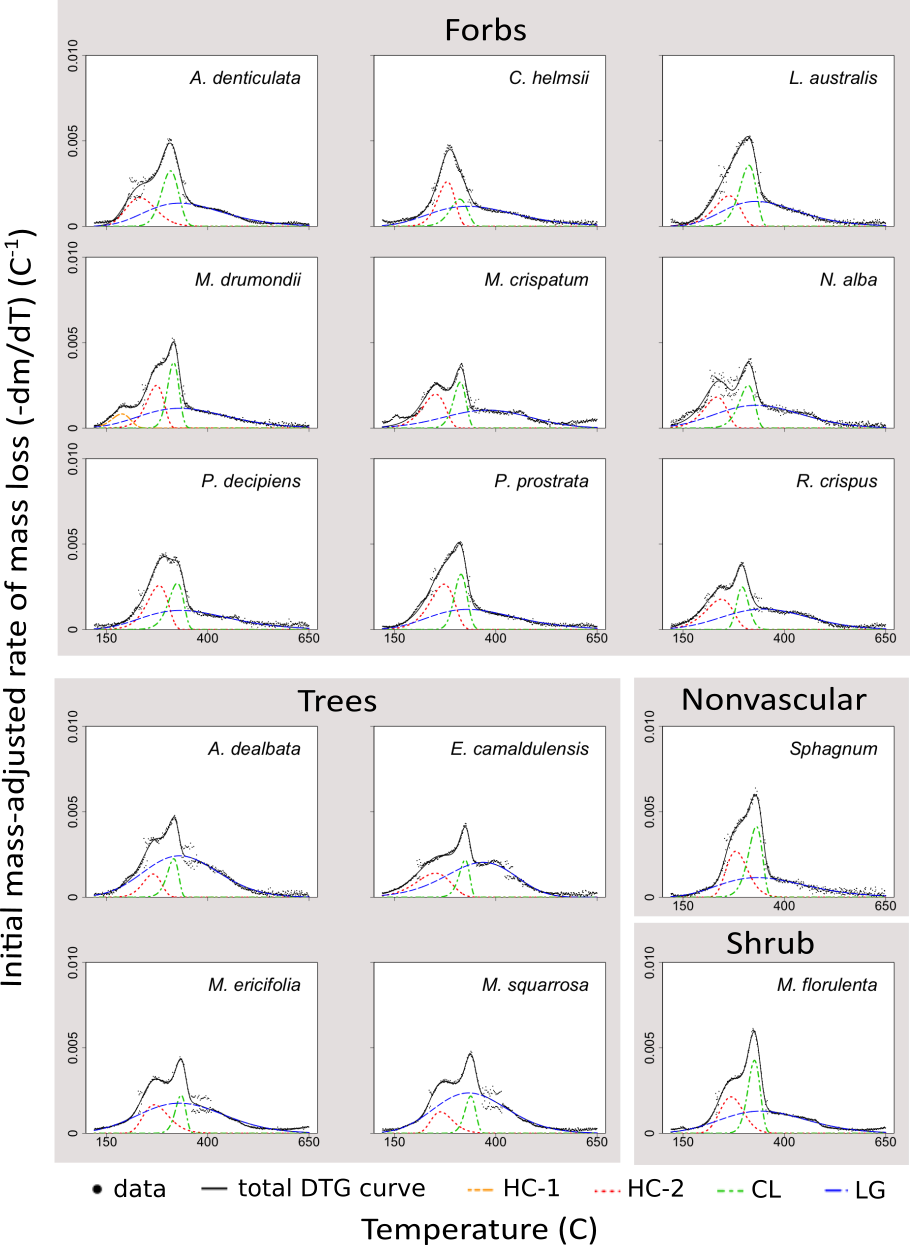
\includegraphics[width=\textwidth]{figs/TGA_fig_other_gfs.png}}
	\caption{Output of deconvolution of thermogravimetric analysis curves. Rate of mass loss (DTG) values scaled by initial mass of sample.}
	\label{Fig:tga_cont}
\end{figure}

\afterpage{%
	\clearpage%
	\thispagestyle{empty}
	\begin{landscape}%
	\centering
		\begin{table}[!ht]
		\caption{Trait values for all species. Economic spectrum trait values represent the average of 10 separate samples. Biomass traits represent the estimates from the pooled biomass of all 10 litter samples with lower and upper confidence intervals of model estimates in brackets.} 
		\label{Tab:speciestraits} 
			\begin{tabular}{l l l r r r r r r r r} 
			\toprule
			\multicolumn{3}{c}{} & \multicolumn{4}{l}{Economic spectrum traits} & \multicolumn{4}{l}{Biomass traits}\\\cmidrule(lr){4-7}
\cmidrule(lr){8-11}
Species & Family & Growth form & \thead{SLA\\ (m$^2$/g)} & \thead{DMC\\ (mg/g)} & \thead{N\\ (wt\%)} & \thead{C\\ (wt\%)} & \thead{HC-1\\ (wt\%)} & \thead{HC-2\\ (wt\%)} & \thead{CL\\ (wt\%)} & \thead{LG\\ (wt\%)} \\ 
			\midrule
 \textit{Acacia dealbata} & Fabaceae & tree & 0.60 & 365 & 3.6 & 50.2 &  & 7.8 [4.7, 12.4] & 8 [4.7, 12.5] & 55.7 [53.3, 58] \\ 
  \textit{Alternanthera denticulata} & Amaranthaceae & forb & 0.54 & 275 & 1.3 & 41.2 &  & 15.6 [8.4, 26.1] & 17.4 [13.1, 22.4] & 32.7 [26.3, 39.1] \\ 
  \textit{Baumea articulata} & Cyperaceae & graminoid & 0.20 & 322 & 0.6 & 44.9 &  & 21.7 [20, 23.7] & 21.5 [20.1, 23.2] & 28.4 [26.7, 30] \\ 
  \textit{Baumea rubiginosa} & Cyperaceae & graminoid & 0.24 & 405 & 0.2 & 42.1 &  & 24.5 [22.8, 26.1] & 17 [16.3, 17.8] & 27 [25.6, 28.3] \\ 
  \textit{Carex appressa} & Cyperaceae & graminoid & 0.26 & 396 & 0.5 & 42.3 &  & 20.6 [18.9, 22.3] & 20 [18.6, 21.6] & 27.7 [25.9, 29.5] \\ 
  \textit{Carex fascicularis} & Cyperaceae & graminoid & 0.45 & 300 & 0.8 & 42.2 &  & 15.9 [13.5, 18.3] & 18.5 [16.8, 20.6] & 27.1 [24.9, 29.3] \\ 
  \textit{Crassula helmsii} & Crassulaceae & forb & 1.48 & 97 & 0.8 & 36.4 &  & 14.2 [0.6, 29.7] & 8.7 [0, 29.8] & 31.3 [29.5, 33.3] \\ 
  \textit{Cycnogeton procerum} & Juncaginaceae & graminoid & 0.90 & 101 & 3.2 & 37.6 &  & 9 [7.9, 10.2] & 11.6 [10.7, 12.5] & 37.9 [36.1, 39.7] \\ 
  \textit{Cyperus eragrostis} & Cyperaceae & graminoid & 0.42 & 253 & 0.6 & 40.5 & 5.7 [4.9, 6.7] & 25.3 [21.5, 29.4] & 13 [12.1, 14] & 22.9 [18.3, 27.5] \\ 
  \textit{Eleocharis acuta} & Cyperaceae & graminoid & 0.94 & 158 & 1.6 & 41.0 &  & 14.5 [12.5, 16.5] & 18.2 [16.4, 20.1] & 31.9 [30.3, 33.6] \\ 
  \textit{Eucalyptus camaldulensis} & Myrtaceae & tree & 0.72 & 453 & 1.4 & 48.5 &  & 15.1 [10, 21.5] & 7.2 [5.2, 9.7] & 44 [37.2, 49.5] \\ 
  \textit{Gahnia filum} & Cyperaceae & graminoid & 0.22 & 433 & 0.2 & 44.1 &  & 22 [0.9, 57.7] & 21.8 [1.8, 68.5] & 27.9 [25.9, 29.9] \\ 
  \textit{Juncus amabilis} & Juncaceae & graminoid & 0.15 & 451 & 0.8 & 45.3 &  & 21.6 [20.4, 22.7] & 17.7 [16.7, 18.7] & 30.5 [29.3, 31.6] \\ 
  \textit{Juncus procerus} & Juncaceae & graminoid & 0.26 & 352 & 0.5 & 43.1 &  & 20.5 [18.3, 22.9] & 13.3 [12.4, 14.2] & 32.1 [30, 34] \\ 
  \textit{Lycopus australis} & Lamiaceae & forb & 0.88 & 326 & 0.9 & 45.3 &  & 14.4 [0.9, 63] & 18.8 [0, 45.3] & 34.1 [21, 45.9] \\ 
  \textit{Marsilea drummondii} & Marsileaceae & forb & 2.27 & 209 & 1.0 & 42.5 & 4.8 [2.8, 6.9] & 13.8 [6.1, 23.6] & 13.8 [6.7, 25.1] & 30.8 [26, 35.8] \\ 
  \textit{Melaleuca ericifolia} & Myrtaceae & tree & 0.22 & 456 & 0.8 & 46.7 &  & 13.2 [10.3, 16.7] & 7.2 [6.2, 8.3] & 46.2 [43.4, 48.8] \\ 
  \textit{Melaleuca squarrosa} & Myrtaceae & tree & 0.18 & 489 & 0.7 & 49.2 & 1.4 [0.1, 34.7] & 8.1 [5.4, 25.1] & 7 [6.2, 8.4] & 52.8 [25.3, 59.1] \\ 
  \textit{Meuhlenbeckia florulenta} & Polygonaceae & shrub & 0.09 & 546 & 0.9 & 45.0 & 1.5 [0.1, 8] & 19.3 [10.8, 30.7] & 16.1 [14, 18.5] & 29.6 [18.4, 39.3] \\ 
  \textit{Myriophyllum crispatum} & Haloragaceae & forb & 0.53 & 180 & 1.1 & 39.3 & 6.9 [0.2, 31] & 14.2 [1.1, 23.6] & 9.2 [5.7, 12.8] & 23.5 [17.9, 28.5] \\ 
  \textit{Nymphaea alba} & Nymphaeaceae & forb & 1.50 & 186 & 2.8 & 42.7 &  & 13 [9.9, 16.5] & 12.3 [10.4, 14.6] & 35.1 [30, 40.1] \\ 
  \textit{Paspalum distichum} & Poaceae & graminoid & 0.07 & 283 & 0.3 & 40.4 &  & 17.9 [7.1, 30.6] & 26.5 [16.3, 39.8] & 22.2 [20.2, 24.4] \\ 
  \textit{Persicaria decipiens} & Polygonaceae & forb & 0.95 & 176 & 0.6 & 43.7 &  & 17.2 [2.2, 36.4] & 13 [0.7, 36.5] & 29.8 [27.2, 32.8] \\ 
  \textit{Persicaria prostrata} & Polygonaceae & forb & 0.97 & 227 & 1.1 & 44.8 &  & 20.6 [5.7, 35.6] & 12.8 [1.4, 34.8] & 31.5 [27.2, 35.6] \\ 
  \textit{Phragmites australis} & Poaceae & graminoid & 0.19 & 480 & 1.2 & 44.6 &  & 18.9 [17.1, 20.9] & 18.3 [17.2, 19.5] & 33.1 [31.7, 34.6] \\ 
  \textit{Restio tetraphyllus} & Restionaceae & graminoid & 0.35 & 443 & 0.1 & 46.2 &  & 22.4 [21.4, 23.4] & 18.5 [17.8, 19.1] & 31.1 [30, 32.3] \\ 
  \textit{Rumex crispus} & Polygonaceae & forb & 2.25 & 87 & 2.1 & 39.1 &  & 15.4 [11.9, 19.8] & 9.3 [7, 11.7] & 31.6 [26, 36.3] \\ 
  \textit{Sphagnum sp} & Sphagnaceae & nonvascular & 0.54 & 519 & 0.4 & 43.0 &  & 17.9 [13.5, 22.8] & 18.4 [15.3, 22.2] & 30.6 [28.6, 32.5] \\ 
  \textit{Typha domingensis} & Typhaceae & graminoid & 0.45 & 288 & 1.0 & 43.9 &  & 14.3 [12.8, 15.9] & 15.5 [14.7, 16.4] & 35.7 [34.4, 37.1] \\ 
  
			\bottomrule
			\end{tabular} 
		\end{table} 
	\end{landscape}
	\clearpage%}
}

\subsection{Economic spectrum traits}
CONDENSE THIS SECTION

Specific litter area (SLA) varied considerably among the 29 species studied. The lowest measured was for the grass, \textit{P. distichum} (0.07 m$^2$/g; Table~\ref{Tab:speciestraits}), and highest for the aquatic fern, \textit{Marsilea drumondii} (2.27 m$^2$/g; Table~\ref{Tab:speciestraits}). Despite the wide variation among forbs, nearly every forb species had higher SLA than species of other growth forms (Fig.~\ref{Fig:SLAboxplot}). This variation perhaps reflects the wide diversity of plant functional types contained within the forb grouping, which includes obligate aquatics such as the water lily \textit{Nymphaea alba}, mud-flat specialists such as \textit{Persicaria decipiens}, and erect perennials such as \textit{Lycopus australis}. Graminoids, trees, the shrub, and the bryophyte had nearly uniformly low SLA.

Litter dry matter content (DMC) was uniformly high for the trees, shrub, and bryophyte, and low for the forbs (Fig.~\ref{Fig:DMCboxplot}). Graminoids varied widely, however, with species encompassing values along almost the entire range. The lowest DMC overall was for the exotic perennial herb, \textit{Rumex crispus} (87.026 mg/g; Table~\ref{Tab:speciestraits}), and highest for the lignum shrub, \textit{Meuhlenbeckia florulenta} (546.462 mg/g; Table~\ref{Tab:speciestraits}). Greater variation in DMC than SLA for graminoids may reflect the similarity in from of these species, but variation in underlying chemistry. The graminoid grouping comprised species that varied strongly in structure, from the diminutive grass, \textit{Paspalum distichum}, to the highly aerenchymatic sedge, \textit{Baumea articulata}, and the strappy blades of the Cumbungi, \textit{Typha domingensis}.

Litter N was overall quite low, with the maximum across species just 3.6 wt\% for the Australian native tree, \textit{A. dealbata} (Table~\ref{Tab:speciestraits}). The lowest value measured was for a dampland sedge, \textit{Restio tetraphyllus} (0.1 wt\%; Table~\ref{Tab:speciestraits}). With the exception of the obligate aquatic, \textit{Cycnogeton procerum}, in general N was lowest for graminoids, and both slightly higher and more variable for forbs and trees (Fig.~\ref{Fig:Nboxplot}). Litter C had comparably low variation between species, and followed fairly consistent pattern increasing from forbs to graminoids and the bryophyte, to the shrub and trees (Fig.~\ref{Fig:Nboxplot}). The lowest C overall was for the obligate aquatic species, \textit{Crassula helmsii} (54.871 mg/g; Table~\ref{Tab:speciestraits}), and highest for the native tree, \textit{A. dealbata} (76.741 mg/g; Table~\ref{Tab:speciestraits}). 

\begin{figure}
\centering
	\begin{subfigure}[!ht]{0.3\textwidth}
		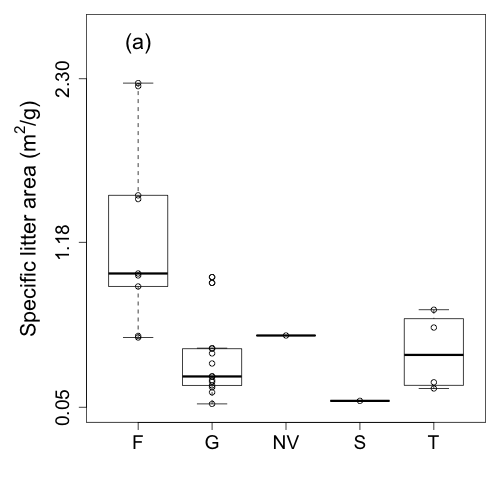
\includegraphics[width=\textwidth]{figs/SLA_boxplot.png}
		\phantomcaption{\label{Fig:SLAboxplot}}
	\end{subfigure}
	\begin{subfigure}[!ht]{0.3\textwidth}
		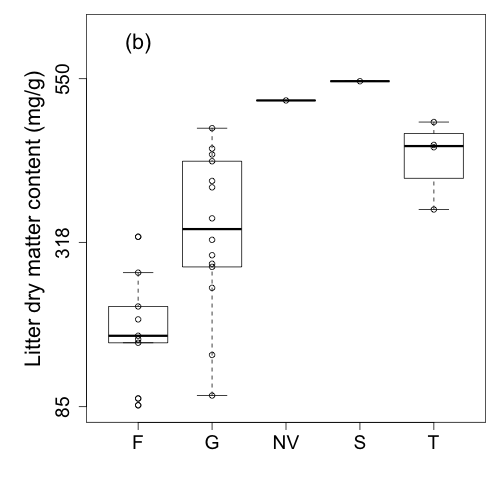
\includegraphics[width=\textwidth]{figs/DMC_boxplot.png}
		\phantomcaption{\label{Fig:DMCboxplot}}
	\end{subfigure}
	\begin{subfigure}[!ht]{0.3\textwidth}
		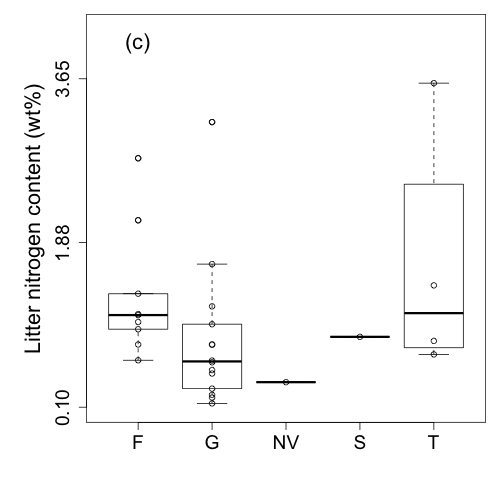
\includegraphics[width=\textwidth]{figs/N_boxplot.png}
		\phantomcaption{\label{Fig:Nboxplot}}
	\end{subfigure}
	\smallskip
	\begin{subfigure}[!ht]{0.3\textwidth}
		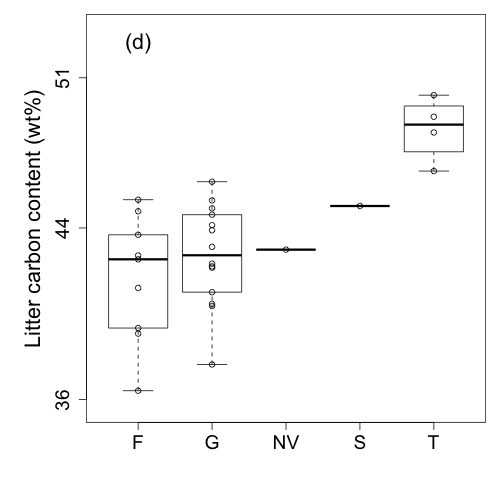
\includegraphics[width=\textwidth]{figs/C_boxplot.png}
		\phantomcaption{\label{Fig:Cboxplot}}
	\end{subfigure}
	\begin{subfigure}[!ht]{0.3\textwidth}
		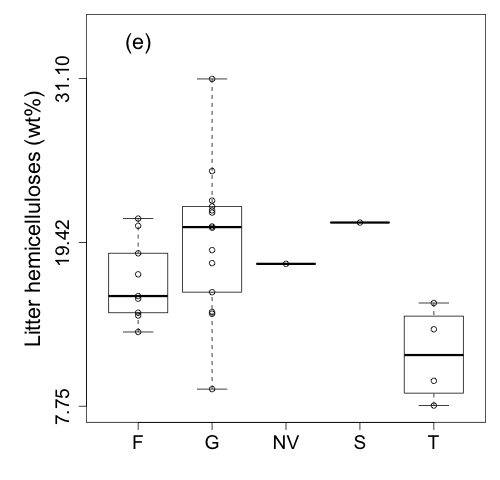
\includegraphics[width=\textwidth]{figs/HC_boxplot.png}
		\phantomcaption{\label{Fig:HCboxplot}}
	\end{subfigure}
	\begin{subfigure}[!ht]{0.3\textwidth}
		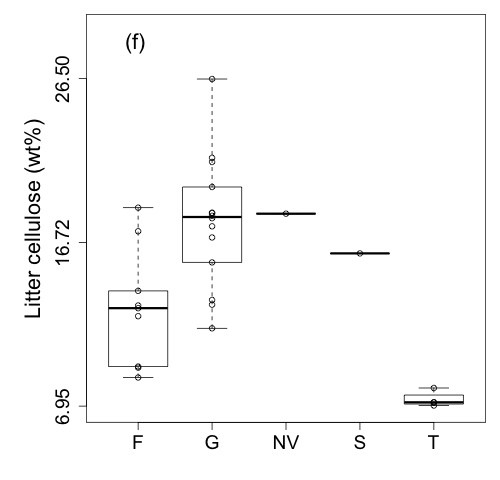
\includegraphics[width=\textwidth]{figs/CL_boxplot.png}
		\phantomcaption{\label{Fig:CLboxplot}}
	\end{subfigure}
	\smallskip
	\begin{subfigure}[!ht]{0.3\textwidth}
		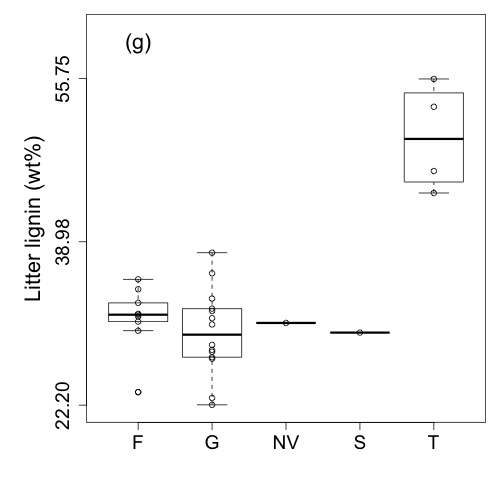
\includegraphics[width=\textwidth]{figs/LG_boxplot.png}
		\phantomcaption{\label{Fig:LGboxplot}}
	\end{subfigure}
	\begin{subfigure}[!ht]{0.6\textwidth}
		\vspace{10 pt}
		\fillcaption{Boxplots of traits by growth form: (a) Specific litter area (m$^2$/g); (b) litter dry matter content (mg/g); (c) litter nitrogen content (wt\%); (d) litter carbon content (wt\%); (e) litter hemicelluloses (wt\%); (f) litter cellulose (wt\%); (g) litter lignin (wt\%). Forbs (herbs and ferns, F; n = 9), graminoids (G; n = 15), non-vascular (NV; n = 1), shrubs (S; n = 1), and trees (T; n = 4). Bold lines represent median values, boxes represent the interquartile range, or middle 50\% of the data, and whiskers represent minimum and maximum values within 1.5 times the interquartile range.}
		\end{subfigure}
\end{figure}

\subsection{Litter traits phylogeny}
Results of the phylogenetic comparison suggest limited evolutionary conservation of trait values. Only SLA has significant ($P$ = 0.01; Table~\ref{Tab:mantel}) correlation with patristic distance, indicating that those with closer relatives have similar SLA, especially among graminoids. Phylogenies are provided in Figs.~\ref{Fig:phyDMC}, \ref{Fig:phyLNC}. 

\begin{figure}[!ht]
	\centering
	\scalebox{0.5}
	{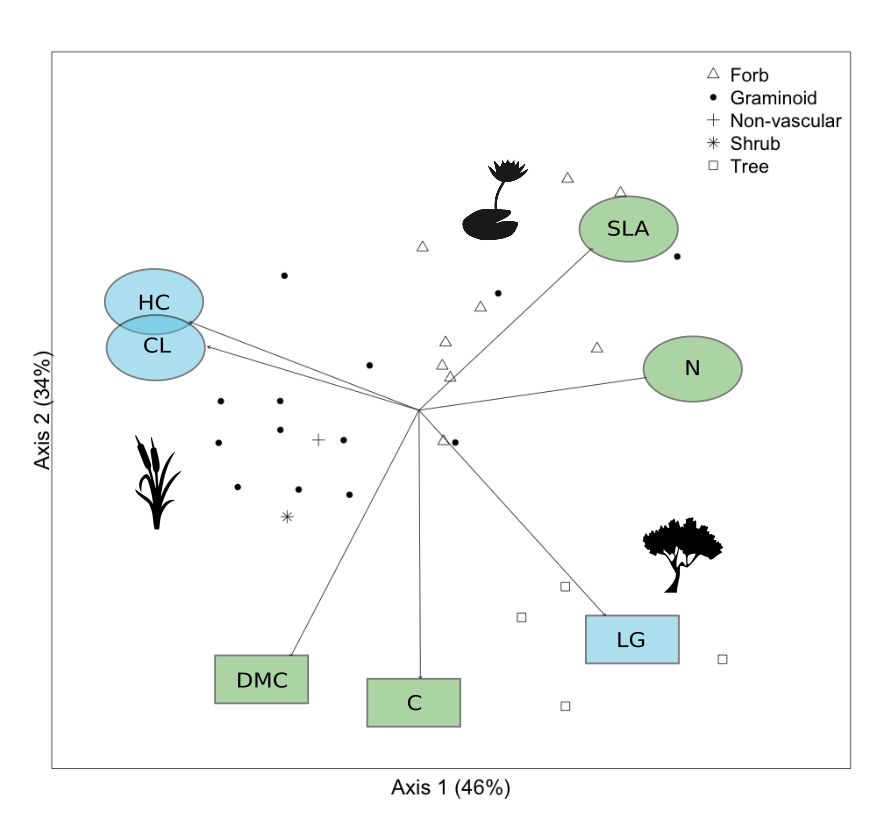
\includegraphics{figs/pca.png}}
	\caption{Principal Component Analysis of traits. Traits standardised and centred prior to ordination.}
	\label{Fig:pca}
\end{figure}

\subsection{Multivariate patterns between economic spectrum and biomass traits}
CONDENSE
The first two axes of the PCA accounted for 80\% of total variation among the species (46\% and 34\%, respectively), and we can see a degree of orthogonality between the economic spectrum traits (SLA, DMC, N, and C; represented in green), and the biomass traits (HC, CL, and LG; represented in blue; Fig.~\ref{Fig:pca}). SLA correlates negatively with DMC by $R^2$ = -0.72, HC and CL similarly negatively correlated with LG by -0.80 and -0.65, respectively (Fig.~\ref{Fig:pairplot}). These two trait axes do not align with the principal component axes, however, indicating that neither economic spectrum nor biomass traits fully dominate the variance among species. Axis 2, representing 34\% of variation can be conceived as separating species by the recalcitrance of their tissue (visualised with trait label shapes; Fig.~\ref{Fig:pca}). The rectangular-shaped trait labels correspond to a suite of both economic spectrum (DMC and C) and biomass (LG) traits that are tightly related to one another (DMC with C 0.75, C with LG 0.59; Fig.~\ref{Fig:pairplot}) and occupying a distinct lower portion of the axis. The round shaped trait labels correspond to those on the opposite end of axis 2, and appear to represent two alternative dominant strategies for non chemically-dense litter. Axis 1 separates these two groupings considerably, separating those with fleshy, high N litter (correlation between SLA and N is 0.52) from those with investment in alternative structural tissue, such as hemicelluloses and cellulose (correlation between HC and CL is 0.52; and N to HC and CL at -0.65 and -0.49, respectively; Fig.~\ref{Fig:pairplot}). 

Growth forms appear clustered, with tree species aligned with the lignin vector, graminoids in the bottom left, characterised by higher DMC and cellulose, and forbs clustered in the upper right, best described by high SLA and N (Fig.~\ref{Fig:pca}). 

\section{Discussion}
In this paper we used thermogravimetric analysis in combination with curve deconvolution to estimate the partitioning of carbon in a suite of wetland plants. We used these biomass traits to identify relationships between traditional leaf traits and recalcitrance. While other work has found that key leaf traits vary along a single dominant axis \citep{wright2005}, we found that species allocate structural carbon into either predominantly cellulose based or lignin based carbon, and that variation in investment of structural carbon is orthogonal to variation in other traits. 

REFER TO ACTUAL RESULTS RATHER THAN PYRAMID - REWRITE
Our results suggest that there is considerable separation among traits into three main clusters. The bottom half of our pyramid (square traits) represents investment in recalcitrant tissue, where the top half (round traits) represents investment in labile tissue. The top half of the pyramid is further divided into two main clusters of traits that divide economic spectrum traits from biomass traits. This division suggests that labile tissue is either dominated by simple carbon carbon forms for by nutrient-rich tissue. >> ADD REF TO NEGATIVE CORR BETWEN HC C AND N

This additional degree of separation would suggest that by measuring biomass traits, we are able to separate species into more complicated groupings than suggested by the single axis model. This makes intuitive sense for the species we see occupying this space. Graminoid species lack chemically complex carbon forms such as lignin, but do invest in significant structural material in the form of high cellulose levels. These tissues serve both photosynthetic and structural purposes, and it is clear from the inclusion of this more comprehensive examination of the traits related to recalcitrance that a considerably more complex picture emerges concerning investment by plants in structural material. The results seem to indicate that plants either invest in cellulose or lignin-dominanted structural tissue, and what's more, this investment strategy does not still align with the division in investment of high or low-quality litter tissue. 

\begin{itemize}
	\item consistency of trait-decomposabililty relationships
	\item across organs
	\item importance of structural tissue traits. 
	\item need to easy to measure way to include these structural traits in future trait studies
	\item the other benefit is that broader biomass traits, allow examining many forms of structure. different components of cell walls. 
	\item lignin may have closest tie to functions like recalcitrance and decomposition, but easy to measure way to get hc and cl could be useful for other functional relationships too. .... 
	\item find studies that looked at hc and cl. hypothesise their relevance. 

\end{itemize}

Across species and growth forms, hemicelluloses dominate mass loss at the lower temperature range, since their simple sugar monomers have random, amorphous structure with little strength, and are easily hydrolysed. which likely corresponds to presence of a different type of simple sugar, such as xylan, amylose, starch, or other derivatives \citep{muller-hagedorn2007}. Cellulose forms long polymers of glucose units without many branches. These linear crystals are more stable, and more resistant to hydrolysis than simple sugars, and so degrade at a higher temperature. However, once temperatures reach past 315 $^{\circ}$C \citep{muller-hagedorn2007}, these chains degrade fairly quickly. Composed of three kinds of heavily-linked benzene-propane, thermal stability of lignin is high, and as such it is more difficult to decompose. Our values for the position of lignin curves match reasonable expectations, since lignin typically decays over a wide temperature interval, and in general dominates mass loss above 400 $^{\circ}$C \citetext{Fig.~\ref{Fig:rawLG} \citealp{chen2015,cai2013,cai2014,varhegyi2011}}). 

Overall, the economic spectrum traits calculated in this study tie in well with the patterns observed in the literature. Forb species had the highest SLA (1.26 compared to 0.36 (G) and 0.43 m$^2$/g (T); Fig.~\ref{Fig:SLAboxplot}), reflecting their place in the economic spectrum containing fast-growing, nutrient rich litter. Slower-growing, nutrient-poor species such as grasses, sedges, reeds, and trees tended to have lower SLA, and higher DMC (333 (G) and 441 (T) compared to 196 mg/g (F); Fig.~\ref{Fig:boxplots}) and C (42.7 (G) and 48.6 (T) compared to 20.5 wt\% (F); Fig.~\ref{Fig:boxplots}). 
While many of the traits displayed patterns by growth form that we would expect, in many cases there was still substantial variation within groupings, suggesting these traits are not very well conserved across growth form. 

\citet{wright2004} acknowledge in a follow-up study that the core relationships outlined in the leaf economic spectrum are not universal, and exhibit a degree of heterogeneity \citep{wright2005}. In an important review of the applicability of trait-based frameworks in wetland ecosystems, \cite{moor2017} note that wetlands contain a different set of constraints on species' strategies than terrestrial systems, which may affect how species segregate along axes of variation. ...

\citet{freschet2012} conclude a complementarity of lignin and dry matter content in predicting litter decompoisiotn, they conldude that this is because dry matter content better captures the proportion of dense to light tissues. This approach may allow us to further break this down, and diagnose that it is the relative proportion of different structural tissues that is in fact driving this difference. DMC correlated strgongly with LG + CL. Perhaps indicating that it encompasses one or both approaches. 



\subsection{Thermogravimetric analysis for biomass trait estimation}
TOO INTRODUCTORY-Y
The TGA and mixture modelling approach, complemented by a freely available software, are a reasonably accessible and affordable approach to begin to quantify biomass traits in naturally-occurring species. Deconvolving DTG curves is a well-established method for estimating biomass fractions in the biofuel field (Orfao and Figueiredo 2001, Barneto et al 2009, Cai and Liu 2007, Chen et al 2017, Orfao et al 1999). Barneto et al 2011 used TGA to characterise the lignocellulosic composition of Eucalyptus wood, and found comparable percent weight contributions as other studies that measured from scratch (Brito et al 2008). 

Across the board, the deconvolution mixture model produced satisfactory mean estimates. For some species, however, the shape of the DTG curve was less confidently resolved, introducing wide confidence intervals in the weight estimates. This error could result from a range of factors: biological or methodological variation, or DTG shape that is simply less identifiable due to sensitivity to starting values or specification of parameter distribution. Using the central tendency, in this case the mean, for estimation of these biomass attributes has produced reasonably confident estimates, particularly considering the quick, and cost-effective characteristics of the method, but future work should test alternative means to clarify and standardise the methodology to other methods of biomass estimation. 

\subsection{Patterns among the other traits -- this is a bad subsection title...}
Overall this suite of wetland species displayed considerable variation in the shape of their DTG curves. While \citet{dedeyn2008} claim that plant traits involved in carbon and nutrient cycling are strongly coupled across functional groups and growth forms, this was not so obvious in our data. 

An important caveat is that our interest was in litter; it would be interesting to repeat the comparisons in this study with just leaves, so as to compare with the leaf economic spectrum more overtly. 

what effect does plant part have
Ex. Marsilea - maybe more cellulose because included the little stem. 
With respect to traits that may affect C donor level/strategy, examining the entire green tissue that would be left behind to be deposited is important. 
nutrient allocation to tissue is not constant within a species, or over time. species grown in different conditions will exhibit different proportions \cite{fornara2012}. 

LES traits tied reasonably with growth form. 
SLA both highest and most variable among forbs.
dry matter highest among woody, most variable among graminoids
nitrogen not clear pattern. 
carbon rising as expected, f g nv s t. 
expected hc to be highest among forbs, but quite variable. 
cellulose was indeed highest among graminoid species, and lignin predictably hiest among the woody trees. 
main takeaway: traits not always well conserved over growth form 


We can conclude that there are no strong evolutionary patterns driving partitioning of carbon types, though additional work following up on evolution of recalcitrance in tissue would be valuable. 

\subsection{Future work}

The current work has begun to identify how different types of species cluster with respect to tissue investment in recalcitrant versus labile tissue, and labile tissue dominantly composed of simple sugars versus those that are more fleshy, and nutrient-rich. Future work should seek to more clearly identify how these trait respond or correlate to environmental conditions, allowing us to link environmental change to variation in authochthonous litter recalcitrance. (this is weak I realise -- main idea, are any of these traits response traits?).

The work conducted here is clearly focused on aboveground plant material. Researchers have already begun to expand the concept of the leaf economic spectrum to include the below ground biomass. Significant work has indicated that belowground biomass not only has a strong effect on biomass contributions to soil carbon, but that the relationships and carbon types of aboveground and below ground litter do not necessarily covary. In addition, belowground root material is typically more carbon complex than aboveground material and therefore may make significant contributions to the volume of recalcitrant litter in the soil. Therefore to get a clear picture of species' contribution to litter quality and soil carbon recalcitrance, biomass trait work will need to examine below ground biomass in the future. 

Future work should also seek to clarify what other ecosystem functions these biomass traits may affect. 

\section{Conclusions}

We found that TGA coupled with modelling approaches is a rapid, low-cost assessment method that can be used to estimate partitioning of litter carbon. The method outlined in this paper, in combination with publicly accessible mixture model code, produce a transparent, reproducible, and relatively affordable method to increase exploration of biomass traits of species, of plant parts, as well as of links to other ecosystem functions. We used this method to identify two alternative strategies for labile tissue, such that there is either investment in simple, easily decomposable carbon forms, or in nutrient-rich tissue. These alternative pathways for labile tissue encompass an additional axis of variation in plant traits, and it remains to be seen how well this pattern holds up in plants from other systems, in other tissue types, and what impacts these compounds have on litter decomposability. 

\section{Acknowledgements}
The authors would like to acknowledge support from the Australian Research Council Centre of Excellence for Environmental Decisions, the Holsworth Wildlife Research Endowment - Equity Trustees Charitable Foundation, and the Melbourne International Research Scholarship and Melbourne International Fee Remission Scholarship from University of Melbourne. We would like to thank the assistance of the University of Melbourne Department of Chemical and Biomolecular Engineering for access to and training on the TGA-FTIR. Vegetation collection was conducted under Victorian Department of Environment, Land, Water and Planning Permit No 10007429. We would like to thank volunteers Paula Sanchez, Abbey Kinnish, Kelsey Johnson, Madeline Brenker, and Urtzi Enriquez Urzelai for assistance in the field collecting plant specimens, Dr Todd McLay for assistance with constructing the species' phylogeny, and acknowledge the besjournals.bst style document. 

\bibliography{../../../bibtex/traits_paper,../../../bibtex/R_packages}

\beginsupplement
\begin{figure}
	\scalebox{0.5}
	{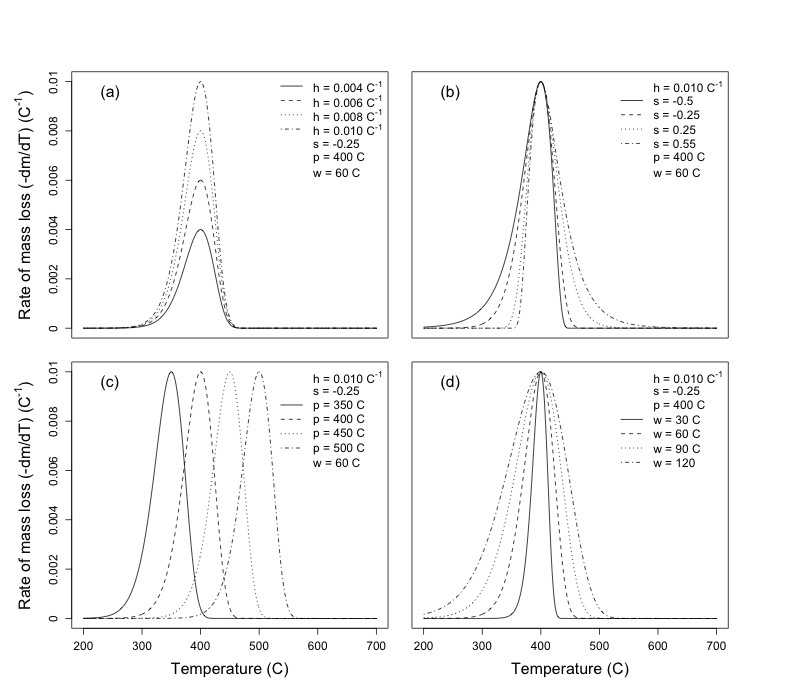
\includegraphics{figs/fs_simulate.png}}
	\caption{Parametric study of the Fraser-Suzuki function for deconvolution of derivative thermogravimetric biomass curves: (a) Effect of modifying height; (b) skew; (c) position; (d) and width.}
	\label{Fig:fs_simulation}
\end{figure}

\afterpage{%
	\clearpage%
	\thispagestyle{empty}
	\begin{landscape}%
	\centering
		\begin{table}[!htbp]
		\caption{Fraser-Suzuki mixture model parameter estimates for each species.} 
		\label{Tab:parameters} 
		\begin{tabular}{l r r r r r r r r r r r r r r r r} 
		\toprule
		\multicolumn{1}{c}{} & \multicolumn{4}{l}{Height} & \multicolumn{4}{l}{Position} & \multicolumn{4}{l}{Skew} & \multicolumn{4}{l}{Width}\\		
		\cmidrule(lr){2-5}
		\cmidrule(lr){6-9}
		\cmidrule(lr){10-13}
		\cmidrule(lr){14-17}
		Species & HC-1 & HC-2 & CL & LG & HC-1 & HC-2 & CL & LG & HC-1 & HC-2 & CL & LG & HC-1 & HC-2 & CL & LG \\ 
		\midrule
		 Acacia dealbata &  NA & 1.36e-03 & 2.25e-03 & 2.42e-03 &  & 265 & 316 & 330 &  & -0.22 & -0.33 & 0.08 &  & 53.00 & 32.20 & 217 \\ 
  Alternanthera denticulata &  NA & 1.68e-03 & 3.24e-03 & 1.36e-03 &  & 233 & 308 & 330 &  & 0.13 & -0.14 & 0.25 &  & 86.90 & 50.00 & 224 \\ 
  Baumea articulata &  NA & 3.68e-03 & 7.24e-03 & 1.07e-03 &  & 263 & 317 & 330 &  & -0.01 & -0.23 & 0.17 &  & 55.50 & 27.40 & 250 \\ 
  Baumea rubiginosa &  NA & 3.89e-03 & 6.04e-03 & 1.01e-03 &  & 266 & 320 & 330 &  & 0.25 & -0.07 & 0.25 &  & 57.80 & 26.40 & 250 \\ 
  Carex appressa &  NA & 3.37e-03 & 6.81e-03 & 1.05e-03 &  & 268 & 321 & 330 &  & -0.12 & -0.17 & 0.11 &  & 57.00 & 27.40 & 250 \\ 
  Carex fascicularis &  NA & 2.53e-03 & 5.55e-03 & 1.02e-03 &  & 265 & 319 & 330 &  & -0.33 & -0.27 & 0.18 &  & 56.80 & 30.50 & 250 \\ 
  Crassula helmsii &  NA & 2.61e-03 & 1.59e-03 & 1.17e-03 &  & 280 & 311 & 330 &  & -0.25 & -0.26 & 0.25 &  & 50.00 & 50.00 & 250 \\ 
  Cycnogeton procerum &  NA & 1.62e-03 & 3.39e-03 & 1.48e-03 &  & 250 & 308 & 330 &  & -0.33 & -0.33 & -0.10 &  & 50.00 & 30.90 & 250 \\ 
  Cyperus eragrostis & 1.57e-03 & 2.65e-03 & 4.47e-03 & 8.64e-04 & 194 & 269 & 311 & 330 & -0.32 & 0.00 & -0.20 & 0.20 & 33.10 & 90.00 & 27.00 & 250 \\ 
  Eleocharis acuta &  NA & 2.42e-03 & 5.73e-03 & 1.22e-03 &  & 270 & 319 & 330 &  & -0.08 & -0.06 & 0.07 &  & 56.10 & 29.70 & 250 \\ 
  Eucalyptus camaldulensis &  NA & 1.41e-03 & 2.18e-03 & 2.04e-03 &  & 251 & 324 & 369 &  & -0.28 & -0.33 & -0.17 &  & 100.00 & 29.60 & 203 \\ 
  Gahnia filum &  NA & 3.98e-03 & 7.22e-03 & 1.04e-03 &  & 280 & 311 & 330 &  & -0.30 & -0.24 & 0.25 &  & 50.20 & 27.70 & 250 \\ 
  Juncus amabilis &  NA & 3.95e-03 & 5.80e-03 & 1.16e-03 &  & 266 & 317 & 330 &  & 0.12 & 0.01 & 0.09 &  & 51.00 & 28.70 & 250 \\ 
  Juncus procerus &  NA & 2.89e-03 & 4.47e-03 & 1.22e-03 &  & 269 & 322 & 330 &  & 0.22 & 0.05 & 0.10 &  & 65.50 & 27.90 & 250 \\ 
  Lycopus australis &  NA & 1.79e-03 & 3.57e-03 & 1.46e-03 &  & 264 & 312 & 330 &  & -0.33 & -0.30 & 0.25 &  & 73.00 & 47.80 & 217 \\ 
  Marsilea drummondii & 8.30e-04 & 2.50e-03 & 3.84e-03 & 1.16e-03 & 188 & 274 & 316 & 330 & -0.20 & -0.33 & -0.14 & 0.20 & 54.50 & 50.00 & 33.60 & 250 \\ 
  Melaleuca ericifolia &  NA & 1.67e-03 & 2.23e-03 & 1.76e-03 &  & 268 & 334 & 330 &  & 0.25 & -0.23 & 0.10 &  & 72.90 & 29.70 & 250 \\ 
  Melaleuca squarrosa & 1.87e-04 & 1.23e-03 & 2.13e-03 & 2.46e-03 & 153 & 262 & 338 & 330 & 0.20 & 0.16 & -0.20 & 0.20 & 80.00 & 61.30 & 30.30 & 200 \\ 
  Meuhlenbeckia florulenta & 2.58e-04 & 2.42e-03 & 4.30e-03 & 1.21e-03 & 143 & 270 & 326 & 358 & -0.16 & -0.01 & -0.12 & 0.20 & 80.00 & 74.90 & 34.90 & 230 \\ 
  Myriophyllum crispatum & 8.19e-04 & 2.29e-03 & 2.69e-03 & 1.04e-03 & 210 & 259 & 313 & 389 & -0.33 & 0.02 & -0.05 & 0.20 & 80.00 & 58.20 & 32.30 & 213 \\ 
  Nymphaea alba &  NA & 1.82e-03 & 2.50e-03 & 1.34e-03 &  & 234 & 310 & 330 &  & -0.33 & -0.33 & 0.11 &  & 65.30 & 44.40 & 250 \\ 
  Paspalum distichum &  NA & 3.24e-03 & 4.83e-03 & 8.50e-04 &  & 275 & 316 & 344 &  & -0.33 & -0.29 & 0.03 &  & 50.00 & 50.00 & 250 \\ 
  Persicaria decipiens &  NA & 2.58e-03 & 2.71e-03 & 1.12e-03 &  & 280 & 325 & 332 &  & -0.33 & -0.33 & 0.25 &  & 60.10 & 43.10 & 250 \\ 
  Persicaria prostrata &  NA & 2.66e-03 & 3.23e-03 & 1.18e-03 &  & 272 & 314 & 330 &  & -0.33 & -0.11 & 0.25 &  & 70.20 & 37.00 & 250 \\ 
  Phragmites australis &  NA & 2.96e-03 & 6.10e-03 & 1.26e-03 &  & 265 & 321 & 330 &  & 0.14 & -0.18 & 0.11 &  & 59.50 & 27.90 & 250 \\ 
  Restio tetraphyllus &  NA & 4.07e-03 & 5.75e-03 & 1.17e-03 &  & 266 & 330 & 330 &  & 0.25 & -0.10 & 0.25 &  & 50.50 & 30.10 & 250 \\ 
  Rumex crispus &  NA & 1.78e-03 & 2.49e-03 & 1.20e-03 &  & 244 & 296 & 347 &  & -0.33 & 0.13 & 0.10 &  & 79.30 & 34.90 & 250 \\ 
  Sphagnum sp &  NA & 2.69e-03 & 4.14e-03 & 1.15e-03 &  & 280 & 331 & 333 &  & 0.20 & -0.31 & 0.25 &  & 61.60 & 40.40 & 250 \\ 
  Typha domingensis &  NA & 2.03e-03 & 6.25e-03 & 1.38e-03 &  & 270 & 324 & 330 &  & -0.03 & -0.29 & 0.01 &  & 66.30 & 22.70 & 250 \\ 
  
		\bottomrule
		\end{tabular} 
	\end{table} 
\end{landscape}
\clearpage
}

\begin{table}[ht] \centering 
	\caption{Gen Bank Accessions codes.} 
	\label{Tab:genbank} 
	\begin{tabular}{l l l} 
	\toprule
		Species & rbcl & matK \\ 
		\midrule 
		 \textit{Acacia dealbata} & NC\_034985.1 & NC\_034985.1 \\ 
  \textit{Alternanthera pungens} & AY514795.1 & AY270054.1 \\ 
  \textit{Baumea articulata} &  & AM999787.1 \\ 
  \textit{Baumea rubiginosa} &  & AY725940.1 \\ 
  \textit{Carex nigra} & FN668463.1 & GQ469838.1 \\ 
  \textit{Crassula falcata} & AF115594.1 &  \\ 
  \textit{Crassula helmsii} &  & KM360736.1 \\ 
  \textit{Cycnogeton procerum} & KF632824.1 & U80713.1 \\ 
  \textit{Cyperus eragrostis} & KX369451.1 & HM849936.1 \\ 
  \textit{Eleocharis acuta} &  & AM999820.1 \\ 
  \textit{Eleocharis marginulata} & KC123404.1 &  \\ 
  \textit{Eucalyptus camaldulensis} & NC\_022398 & NC\_022398.1 \\ 
  \textit{Gahnia aspera} &  & AB369962.1 \\ 
  \textit{Juncus maritimus} & JN894909.1 & AY216629.1 \\ 
  \textit{Lycopus rubellus} & KJ772924.1 & KJ773662.1 \\ 
  \textit{Marsilea crenata} & KC536646 &  \\ 
  \textit{Marsilea drummondii} &  & DQ643299.1 \\ 
  \textit{Melaleuca leucadendra} &  & KX527090.1 \\ 
  \textit{Melaleuca viridiflora} & AF184708.1 &  \\ 
  \textit{Muehlenbeckia australis} &  & FM883618.1 \\ 
  \textit{Myriophyllum exalbescens} &  & L11195.2 \\ 
  \textit{Myriophyllum sibiricum} & EF178980.1 &  \\ 
  \textit{Nymphaea alba} & AJ627251 & AJ627251 \\ 
  \textit{Paspalum distichum} & FN908063.1 & FN870399.1 \\ 
  \textit{Persicaria decipiens} & KR734365.1 & FM883624.1 \\ 
  \textit{Phragmites australis} & MF035995 & MF035995 \\ 
  \textit{Restio tetraphyllus} & AF164379.1 & AF206816.1 \\ 
  \textit{Rumex crispus} & EU840458.1 & JX848510.1 \\ 
  \textit{Sphagnum australe} & KU725452 & KU725452.1 \\ 
  \textit{Typha domingensis} & HM850522.1 & KJ773961.1 \\ 
  
		\bottomrule
	\end{tabular} 
\end{table} 

\begin{figure}
   \centering
	\begin{subfigure}[h]{0.7\textwidth}
		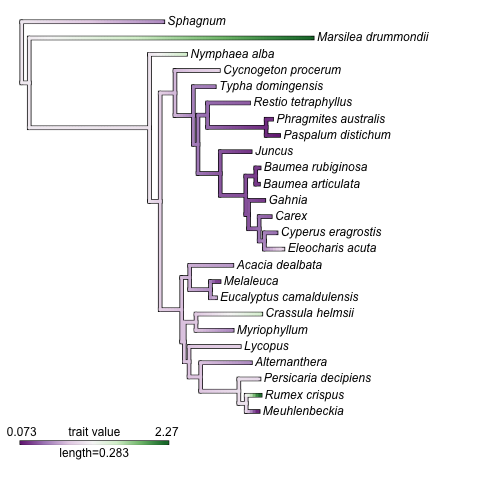
\includegraphics[width=\textwidth]{figs/phylo_SLA.png}
		\caption{Specific litter area (m$^2$/g)}
		\label{Fig:phySLA}
	\end{subfigure} %
	\hfill
	\begin{subfigure}[h]{0.7\textwidth}
		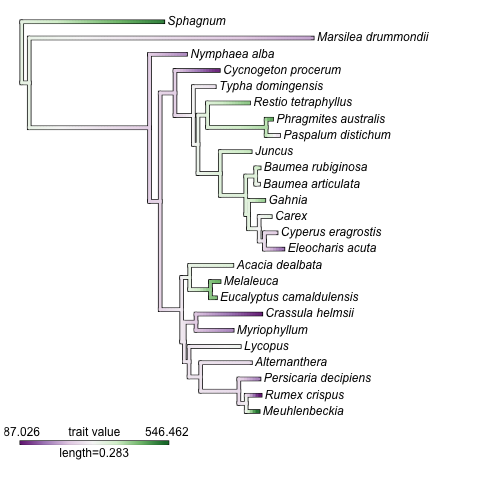
\includegraphics[width=\linewidth]{figs/phylo_DMC.png}
		\caption{Litter dry matter content (mg/g)}
		\label{Fig:phyDMC}
	\end{subfigure}
\end{figure}
\begin{figure}[htb]\ContinuedFloat
    \centering
	\begin{subfigure}[h]{0.7\textwidth}
		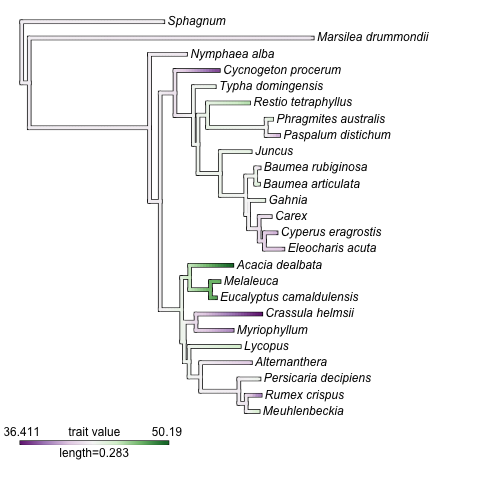
\includegraphics[width=\linewidth]{figs/phylo_C.png}
		\caption{Litter carbon content (wt\%)}
		\label{Fig:phyLCC}
	\end{subfigure} 
	\hfill
	\begin{subfigure}[h]{0.7\textwidth}
		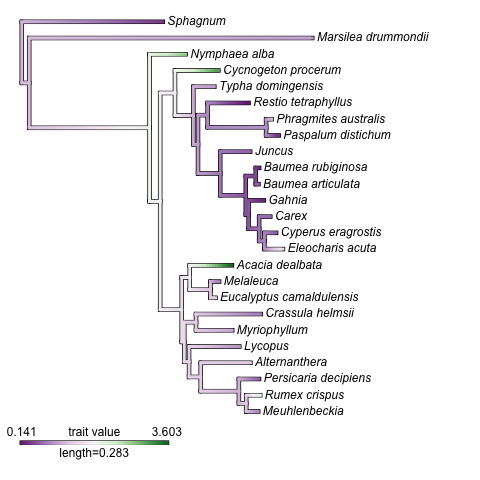
\includegraphics[width=\linewidth]{figs/phylo_N.png}
		\caption{Litter nitrogen content (wt\%)}
		\label{Fig:phyLNC}
	\end{subfigure}	
\end{figure}
\begin{figure}[htb]\ContinuedFloat
    \centering
	\begin{subfigure}[h]{0.7\textwidth}
		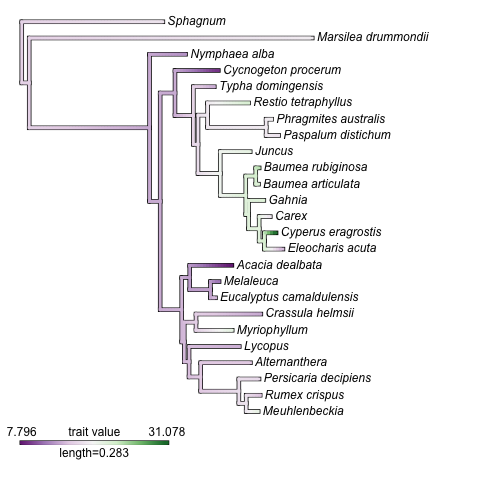
\includegraphics[width=\linewidth]{figs/phylo_HC.png}
		\caption{Litter hemicelluloses content (wt\%)}
		\label{Fig:phyHC}
	\end{subfigure} %
	\hfill
	\begin{subfigure}[h]{0.7\textwidth}
		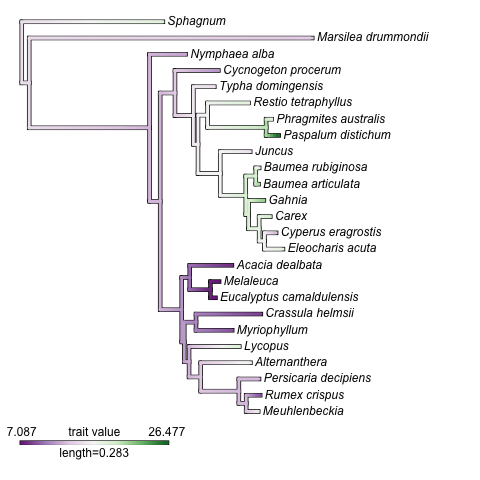
\includegraphics[width=\linewidth]{figs/phylo_CL.png}
		\caption{Litter cellulose content (wt\%)}
		\label{Fig:phyCL}
	\end{subfigure}		
\end{figure}
\begin{figure}[htb]\ContinuedFloat
    \centering
	\begin{subfigure}[h]{0.7\textwidth}
		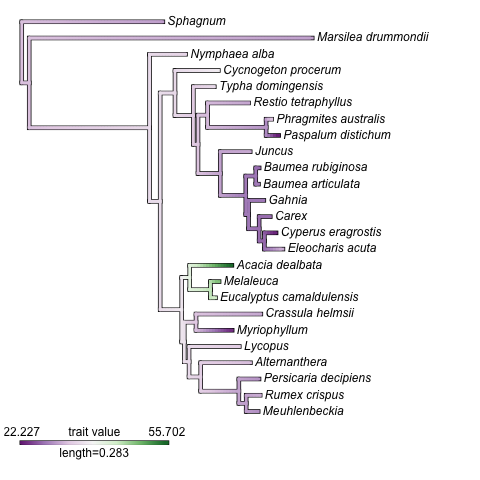
\includegraphics[width=\linewidth]{figs/phylo_LG.png}
		\caption{Litter lignin content (wt\%)}
		\label{Fig:phyLG}
	\end{subfigure} %
	\caption{Phylogenetic tree of species included in this study. Genus level where species level sequences for rcbL gene unavailable. In that case, if represents more than one species, the trait value was averaged between species in that genus.}
\end{figure}	
	
\begin{table}[ht] \centering 
	\caption{Mantel test for the correlation between patristic distance and functional trait differences between the seven selected traits.} 
	\label{Tab:mantel} 
	\begin{tabular}{l r r} 
	\toprule
		Trait & Mantel Test observation & $P$-value \\ 
		\midrule 
		 \textbf{Specific litter area} & \textbf{0.42} & \textbf{0.01} \\ 
  Litter dry matter content & 0.06 & 0.26 \\ 
  Litter nitrogen & -0.1 & 0.71 \\ 
  Litter carbon & -0.13 & 0.85 \\ 
  Litter hemicelluloses & -0.11 & 0.83 \\ 
  Litter cellulose & -0.01 & 0.47 \\ 
  Litter lignin & -0.14 & 0.87 \\ 
  
		\bottomrule
	\end{tabular} 
\end{table} 
	
\begin{figure}
	\scalebox{0.5}
	{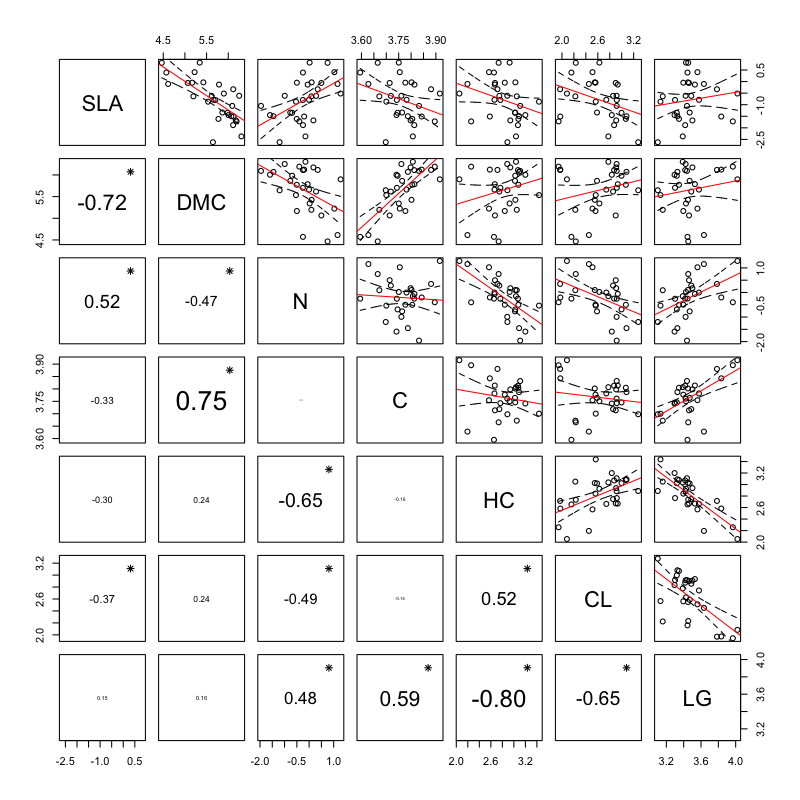
\includegraphics{figs/pairplot.png}}
	\caption{Correlations between traits. Size of $R^2$ listed on bottom panel proportional to weight of relationship, with star to indicate significance at $P$ \textless 0.05.}
	\label{Fig:pairplot}
\end{figure}

\begin{table}[!htbp]\centering
	\caption{Principal Component Analysis axis loadings.}
	\label{Tab:pca}
	\begin{tabular}{l r r r r}
        		\toprule
        		Trait & Axis 1 & Axis 2 \\
        		\midrule  
		 Specific litter area & 0.37 & 0.34 \\ 
  Litter dry matter content & -0.29 & -0.54 \\ 
  Litter nitrogen & 0.47 & 0.07 \\ 
  Litter carbon & 0.00 & -0.61 \\ 
  Litter hemicelluloses & -0.47 & 0.17 \\ 
  Litter cellulose & -0.43 & 0.12 \\ 
  Litter lignin & 0.40 & -0.43 \\ 
  
        		\bottomrule
	\end{tabular}
\end{table}

\begin{figure}
\centering
	\begin{subfigure}[b]{0.48\textwidth}
		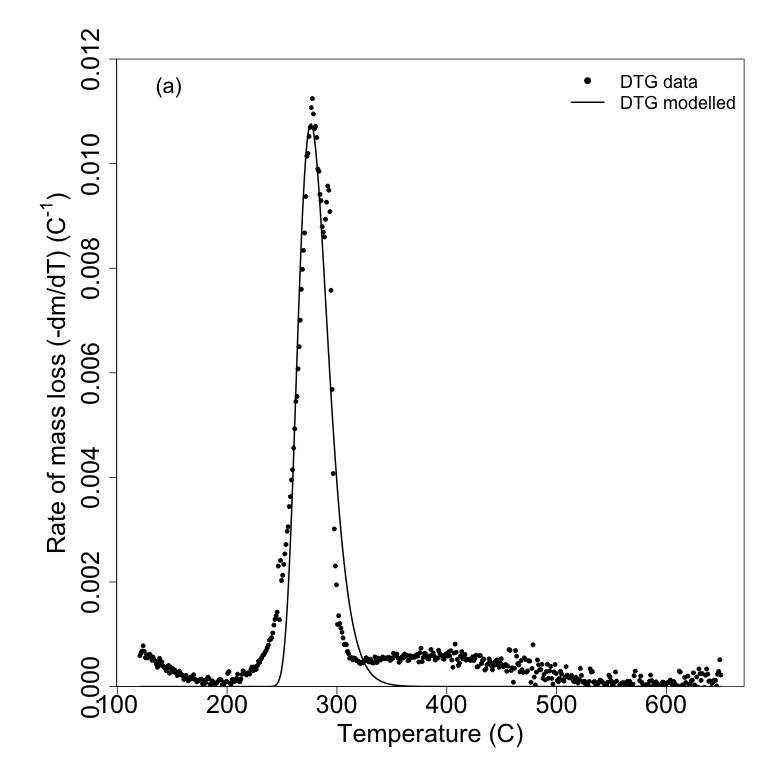
\includegraphics[width=\textwidth]{figs/raw_CL.png}
		\phantomcaption{\label{Fig:rawCL}}
	\end{subfigure}
	\hfill
	\begin{subfigure}[b]{0.48\textwidth}
		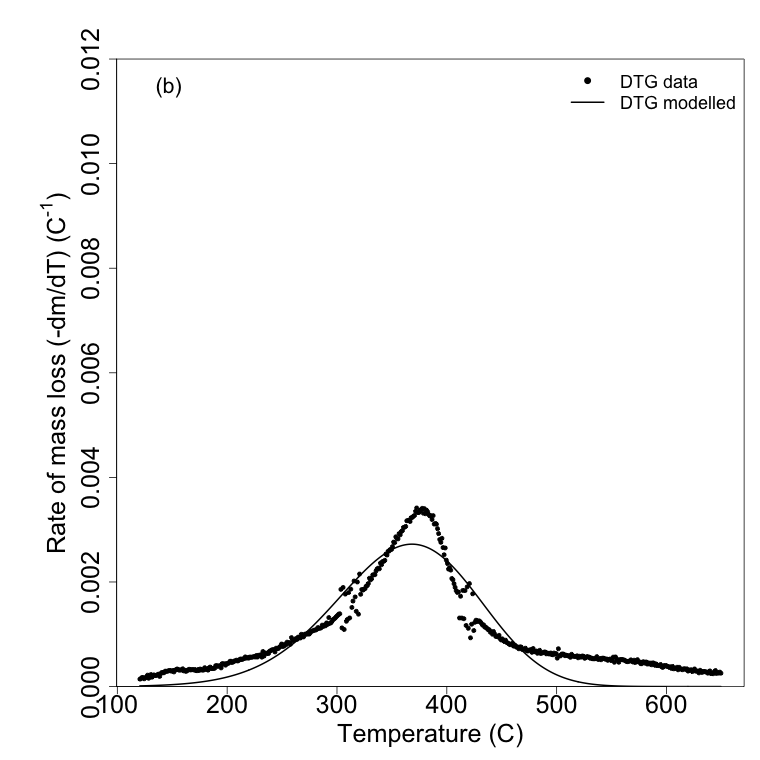
\includegraphics[width=\textwidth]{figs/raw_LG.png}
		\phantomcaption{\label{Fig:rawLG}}
	\end{subfigure}
	\caption{Predicted negative derivative thermogravimetric for raw biomass samples: (a) Carboxy-methyl cellulose raw mass loss data and modelled DTG curve; (b) Lignin raw mass loss data and modelled DTG curve.}
\end{figure}

\end{document}

